\documentclass[11pt]{article}

\newcommand{\squishlist}{
   \begin{list}{$\bullet$}
    { \setlength{\itemsep}{0pt}      \setlength{\parsep}{3pt}
      \setlength{\topsep}{3pt}       \setlength{\partopsep}{0pt}
      \setlength{\leftmargin}{1.5em} \setlength{\labelwidth}{1em}
      \setlength{\labelsep}{0.5em} } }

\newcommand{\squishlistB}{
   \begin{list}{--}
    { \setlength{\itemsep}{0pt}      \setlength{\parsep}{3pt}
      \setlength{\topsep}{3pt}       \setlength{\partopsep}{0pt}
      \setlength{\leftmargin}{1.5em} \setlength{\labelwidth}{1em}
      \setlength{\labelsep}{0.5em} } }

\newcommand{\squishend}{
    \end{list}  }

\usepackage{times}
\usepackage{mathptm}
\usepackage{fullpage}
\usepackage{hyperref}
\usepackage{graphicx}

\begin{document}

\begin{center}
\medskip
{\bf{Regis University -- Physics 305A -- Fall 2019}} \\
{\bf{Lab 4: Impulse and Momentum Change in 1-D}} \\
\medskip

{\em{Derived from activities EX01 and EX02 in the instructor resources that
 accompany \\ Ruth Chabay and Bruce Sherwood's {\em Matter and Interactions} 
 textbook.}}
\medskip
\end{center}

\section{Introducing the ultrasonic motion detector}

You will use a motion sensor to display graphs of the $x$-component of the {\em position} of your hand vs. time and the $x$-component of {\em velocity} of your hand vs. time.  The motion sensor detects the position of an object the same way a bat does.
It emits pulses of ultrasound (sound whose pitch is too high for human
ears to detect), and measures the time required for a pulse to travel to an
object, be reflected by the object, and return to the detector. The speed of
a sound wave in air is about 340 meters per second at room temperature; knowing this, a
computer program can calculate the distance between the object and the
detector, and display this on the graph.  The ticking sound you hear is not
the ultrasound, but is ordinary low-pitched sound; it lets you know the unit
is working.

\squishlist
\item Set up the equipment so that Logger Pro will display two graphs:
\squishlistB
\item $x$-component of position ($x$) versus time
\item $x$-component of velocity ($v_x$) versus time
\squishend
\item Mount the motion sensor at the end of the track.
\item Hold your open hand about a foot in front of the sensor.
\item Start recording, then slowly move your hand away from the sensor, then slowly back toward the sensor.
\item Stop recording and save your graphs.\\
\squishend

Look at your graphs, and make sure you can answer the following questions. If necessary, do further experiments to make sure you understand.\\

\squishlist
\item What location in space is considered to be the origin?
\item In which direction (in your actual experimental setup) does the positive $x$-axis run?
\item To make $v_{x}$ positive, should you move your hand toward the sensor or away from the sensor?
\item What do you have to do to make the graph of $x$ vs. $t$ a horizontal line?
\item What do you have to do to make the graph of $v_{x}$ vs. $t$ a horizontal line?
\squishend

\medskip

The motion sensor does not measure $v_{x}$ directly. The software repeatedly
calculates $v_{x}$ by taking position measurements at two different times,
and calculating $\Delta x/\Delta t$ from these measurements. Therefore, it
is calculating an average $v_{x}$, but since the time between the
measurements is very short, the average $v_{x}$ is a very good approximation
to the instantaneous $v_{x}$.

\newpage

\section{Measuring $x$ and v$_{x}$ for a low-friction cart with the fan off}

\squishlist
\item Place a cart on the track, but do not turn on the fan. The cart rolls on the track with little (but not zero) friction.
\item Try giving the cart a gentle push; find out how hard you have to push it to get it to roll the length of the track in about 3-5 seconds. (Please do not let the cart hit the motion sensor! You may find that you get a cleaner signal if you tape a piece of cardboard to the base of the cart as shown in the picture.)
\squishend

\begin{center}
\vspace{10pt}
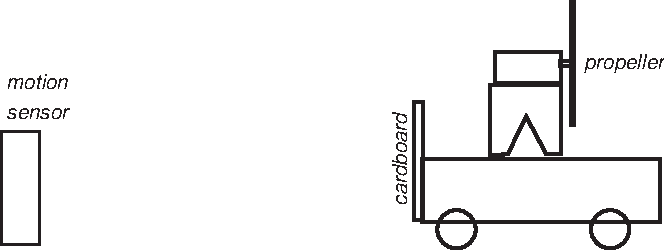
\includegraphics[scale=0.75]{fancart_diagr.pdf}
\end{center}

\squishlist
\item Record a graph of $v_{x}$ vs. $t$ that is approximately like the one below:

\begin{center}
\vspace{10pt}
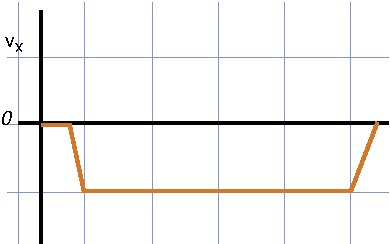
\includegraphics{vx_neg_const.pdf}
\end{center}

\item From your graph, determine:
\squishlistB
\item The cart's average speed while it was moving, and 
\item the magnitude of its average momentum (you will need to measure an additional quantity to get this...which one?) 
\squishend
\squishend

\newpage

\section{Changing velocity and momentum: constant force from fan}

When the fan is turned on, the air exerts a nearly constant force on the
fan cart.

\subsection{$v_x$ positive and increasing}


\squishlist

\item Find initial conditions such that when the fan is turned on, and the cart is
released from rest, the $x$-component of the cart's velocity is positive and
increasing.

\squishlistB
\item What are the initial conditions (position, direction of initial motion, direction of force by air on fan cart) required to produce this motion?
\item What do the graphs of $x$ vs. time and $v_x$ vs. time look like?
\item In a one-second interval, what is $\Delta p_x$?
\item In a two-second interval, what is $\Delta p_x$?
\item What is the net force acting on the fan cart during each of these intervals?
\squishend
\squishend


\subsection{Force opposite to initial velocity}
\squishlist
\item Orient the cart so that the force of the air on the fan cart is in the $-x$
direction. Turn on the fan, start the sensor, then give the cart a shove in
the $+x$ direction.
\squishlistB
\item In a one-second interval while the cart is heading in the $+x$ direction, what is $\Delta p_x$? (Make sure your sign is correct.)
\item In a one-second interval while the cart is heading in the $-x$ direction, what is $\Delta p_x$? (Make sure your sign is correct.)
\item What is the net force acting on the cart during each of these intervals? 
\squishend

\squishend

\squishlist
\item Think about your results in this section of the activity. Do you think $\Delta p_x$ should be the same in both situations (cart heading in $+x$ and $-x$ directions)? Why or
why not? 
\item From your data, do you get the same value or different values for $F_{net,x}$ in the two situations? Why or why not? 
\squishend

\section{Adding a force sensor}

Next, attach a force sensor to the opposite end of the track from the 
motion detector; you will bounce the cart off of it and observe the
relationship between the force exerted on the cart and change in its
momentum.
To see how the equipment works:

\squishlist
\item  Start Logger Pro, then press gently on the spring on the force sensor. Try compressing the spring slowly and rapidly, to see what kind of graph is produced.

\item  If the force does not read zero when the spring is not compressed, there is a button in Logger Pro to zero the reading.

\item  Roll the cart gently so it bounces off the spring on the force sensor; find a speed that produces a clearly visible signal, but does not flatten out at the top, which would indicate a force too large to measure with these settings.

\item  Make sure you understand the graphs of $F_x$ vs. $t$ and $v_x$ vs. $t$ that are produced simultaneously.
\item  Does the graph of $F_x$ vs. \textit{t} show the force on the sensor due to the cart, or the force on the cart due to the sensor? (Think about the sign of $F_x$).
\squishend

The interaction between the cart and the force sensor is due to electric interactions between the protons and electrons in the cart and those in the sensor. It is a property of the electric interaction that the electric forces exerted by two objects on each other are equal and opposite. Therefore, the graph of $F_x$ on the cart versus \textit{t} would be the same as the one you see, but the values of $F_x$ would be negative.

\medskip 

Clearly,  $F_x$ in this experiment is not constant; it varies with time. However an \textit{average} value of $F_x$ can be estimated by examining your graph, which probably looks something like this:

\begin{center}
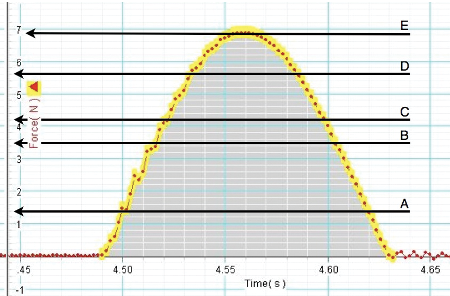
\includegraphics[scale=1.4]{Impulse.pdf}
\end{center}

\squishlist
\item First, determine why $F_x$ is \textit{not} constant. Clearly explain your reasoning.

\item Examine the sample graph above and determine which value (A, B, C, D, or E) best represents the \textit{average} value of $F_x$.
\squishend

\section{Simultaneous measurement of $F_x$ and $\Delta p_x$}

Use your equipment to measure $F_x$ vs. \textit{t} and $v_x$ vs. \textit{t} while the cart rolls toward the force sensor, collides, and bounces off, rolling backward toward your hand. (Please do not let the cart hit the motion sensor.)

\squishlist
\item  From the graph of $v_x$ vs. \textit{t} generated by the motion sensor(along with any other necessary data you may need), determine the change in the \textit{x} component of the cart's momentum from just before the collision starts to just after it ends. Record this as $\Delta p_x$.

\item From your graphs, estimate the total duration of the collision, $\Delta t$.

\item  From the graph of $F_x$ vs. \textit{t} generated by the force sensor, estimate the average value of $F_x$ during this interval.

\item  Using this average value, estimate the impulse $F_x \Delta t$ applied by the sensor on the cart during the collision (with correct sign).

\item  How does your calculated value of $\Delta p_x$ compare to your estimated value of $F_x \Delta t$?

\item  How would you expect these values to compare?\\
\squishend

There is a more accurate way to determine the actual impulse on the cart. In the first short time interval $\Delta t_1$, the spring is only slightly compressed, and the force $F_{x_1}$ on the cart is small. The small impulse $F_{x_1} \Delta t_1$ makes a small change $\Delta p_{x_1}$ in the momentum. But $F_{x_1} \Delta t_1$ can be thought of as the area of a rectangle shown on the diagram, whose base is $\Delta t_1$ and height is $F_{x_1}$. So the area of the rectangle is equal to the impulse during $\Delta t_1$ and also equal to the change in momentum $\Delta p_{x_1}$ during that short time interval.\\

In the next time interval $\Delta t_2$, we can again represent the impulse (and the change in momentum) as the area of the next rectangle shown on the diagram. We can continue through the entire collision with the spring, and we see that the total area under the curve is equal to the total impulse (and the total change in the momentum, which is the sum of all the changes to the momentum). We're approximating the area under the curve by a bunch of rectangles, but if the little $\Delta t$'s are small enough that the force isn't changing much during that short time interval, the total area of our rectangles is approximately equal to the area under the curve.\\

This is an example of an ``integral'', which can often be thought of as the area under a curve. More generally, an ``integral'' is the sum of a large (infinite) number of very small (infinitesimal) quantities. The integral of impulse is written $\int F_{x} \, dt $, where the integral sign is a distorted ``S'' meaning ``sum'' and the ``\textit{dt}'' stands for ``extremely small (infinitesimal) time interval''.

\begin{center}
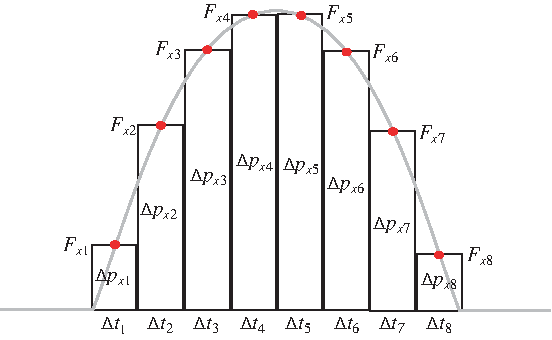
\includegraphics[scale=1]{Ft-integral.pdf}
\end{center}

\squishlist
\item  Logger Pro has an option to calculate the area under the $F_x$ vs. \textit{t} curve for you.
 How does the $x$ component of the net impulse found using $\int F_{x} \, dt $ compare to the $x$ component of the change in the cart's momentum?
 (Remember that the actual value of the impulse applied to the cart is negative).

\item At the instant when $F_x$ is the biggest it ever gets, what is $p_x$? Is $p_x$  also at a maximum at that time, or something else?
\squishend


\end{document}
